%%----------------------------------------------------------
\section{Design}
%%----------------------------------------------------------
  % --------------------
  \begin{figure}
    %
    \begin{center}
      % Replace with pdf fig
      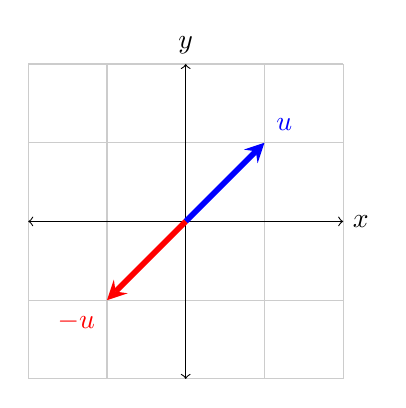
\begin{tikzpicture}
        \draw[thin,gray!40] (-2,-2) grid (2,2);
        \draw[<->] (-2,0)--(2,0) node[right]{$x$};
        \draw[<->] (0,-2)--(0,2) node[above]{$y$};
        \draw[line width=2pt,blue,-stealth](0,0)--(1,1)
              node[anchor=south west]{$\boldsymbol{u}$};
        \draw[line width=2pt,red,-stealth](0,0)--(-1,-1)
              node[anchor=north east]{$\boldsymbol{-u}$};
      \end{tikzpicture}
    \end{center}
    %
    \caption{\label{fig:vectors} Each paper should have a killer
    figure 1 that captures the essence of the approach idea. It
    can happen that figure 1 is a great related work comparison
    and then it will require a second system architecture
    figure.}
  %
  \end{figure}

  % --------------------
  How do we acheive that lofty goal? 
  %
  Well of course by solving several unsolved challenges.
  %
  The section sub headings in this paragraph should roughly
  align with those core original contributions and highlight
  both the overall design and key technical challenges and
  solutions in doing so.

